\section{Proposed Solution}
In this section, I will provide the steps utilized in my study. Because no significant research is there ~\footnote{I did not come across with some search} on finding relations of food groups with ACR where data clustering is also used, we propose a solution to use data clustering and find associations of food groups with ACR. For data clustering, we propose age and CKD-stage-based studies as well as clustering algorithms such as K-means. Various clustering techniques such as consensus clustering is used for CKD-related studies not for Food groups with ACR studies. Other clustering techniques as well as ensembled clustering techniques can be a future candidate. For the project, we propose age and CKD stage-based study as well as clustering algorithms such as K-means.

\subsection{Methodology Overview}
%\subsection {Approach and Steps}
\flushleft \justifying In the project, I have utilized data from NHANES, CDC. I have taken CDC data on Demographics, Dietary surveys, and Laboratory data ~\cite{CDCDataset}. The data exist from 1996 to 2018. In the project, I have utilized data from 2011 to 2018. I have merged Demographics data, Dietary Intake Data, and ACR readings data from different CDC sources to create the dataset to be utilized in this project. Afterward, I have done data exploration and data curation for data types and missing data. I ensured the output dataset contain data only when data exist for an individual for each aspect such as demographics, diet, and ACR readings. At this point, I have clustered i.e. grouped the data into nine different groups based on Age and ACR readings. Afterward, for each group as well as the total dataset, I find out the most important food groups in the dataset. I have utilized Principle Component Analysis (PCA) to find the important food groups. Afterward, I used Statistical analysis and Pearson correlation to find the correlations of food groups with ACR for each cluster/group. The steps in the proposed solution are given in Figure ~\ref{gfr-acr-ckd-methodology}.

\tikzstyle{startstop} = [rectangle, rounded corners, minimum width=2cm, minimum height=1cm,text centered, draw=black, fill=red!30]
\tikzstyle{io} = [trapezium, trapezium left angle=70, trapezium right angle=110, minimum width=2cm, minimum height=1cm, text centered, draw=black, fill=blue!30]
\tikzstyle{process} = [rectangle, minimum width=3cm, minimum height=1cm, text centered, draw=black, fill=orange!30]
\tikzstyle{decision} = [diamond, minimum width=3cm, minimum height=1cm, text centered, draw=black, fill=green!30]
\tikzstyle{arrow} = [thick,->,>=stealth]

\subsection{Overall Architecture Machine Learning Assisted Track Management}
Overall Architecture for Machine Learning Assisted Track Management is given in figure ~\ref{overall-architecture}.
\begin{figure}[!htb]
\begin{tabular}{c}
\begin{tikzpicture}[node distance=1.5cm]
<TikZ code>
\node (start) [startstop] {Start};
\node (surveydata) [io, text width=8cm, below of=start] {CDC/NHANES Survey data on Demographics, Dietary Intake, and ACR results };
\node (acrdata) [io, text width=2.5cm, below of=surveydata, yshift=-0.25cm, xshift=-3cm] {ACR Data};
\node (fooditems) [io, text width=2cm, right of=acrdata, xshift=5cm] {Food Items};
\node (foodgroups) [io, text width=4cm, below of=fooditems] {Food Group Intake};

\node (proceefoodacr) [process, text width=4cm, below of=acrdata] {Merge ACR, Food Group Intake};
\node (sourcefood) [io, text width=4cm, below of=proceefoodacr] {Source: Food Group Intake Target: ACR};
\node (cluster) [process, text width=5cm, below of=sourcefood] {Clustered Groups based on Age and AC level};
\node (regression) [process, text width=5cm, below of=cluster, yshift=-0.25cm] {Regression/Correlation Relate Food Groups with ACR};
\node (corregression) [io, text width=3cm, below of=regression, xshift=-2cm, yshift = -1cm] {Correlated Food Groups with ACR};
\node (ml) [process, right of=corregression, xshift=3cm] {ML Methods};
\node (acrpredict) [process, text width=5cm, below of=ml] {ACR Predictability};
\node (predicted) [io, text width=3cm, below of=acrpredict, xshift=-2cm] {Predicted ACR from Food Intake};
\node (stop) [startstop, below of=predicted] {Stop};



\draw [arrow] (start) -- (surveydata);
\draw [arrow] (surveydata) -- (acrdata);
\draw [arrow] (surveydata) -- (fooditems);
\draw [arrow] (fooditems) -- (foodgroups);

\draw [arrow] (acrdata) -- (proceefoodacr);
\draw [arrow] (foodgroups) -- (proceefoodacr);

\draw [arrow] (proceefoodacr) -- (sourcefood);
\draw [arrow] (sourcefood) -- (cluster);
\draw [arrow] (cluster) -- (regression);
\draw [arrow] (regression) -- (corregression);
\draw [arrow] (regression) -- (ml);

\draw [arrow] (ml) -- (corregression);
\draw [arrow] (ml) -- (acrpredict);
\draw [arrow] (acrpredict) -- (predicted);
\draw [arrow] (predicted) -- (stop);
\end{tikzpicture}
\end{tabular}
\caption{Overall Methodology: (Clustered) Food Groups Relations with ACR}
\label{overall-architecture}
\end{figure}


\subsection {Dataset}
For the study, I have utilized a dataset from NHANES, CDC. I have taken CDC data on Demographics, Dietary surveys, and Laboratory data ~\cite{CDCDataset}. The data exist from 1996 to 2018. In the project, I have utilized data from 2011 to 2018. I have used a semi-automated method to convert the data from CDC to be utilized in this project.


\subsubsection{Data Synthesis}
\noindent Initially, all the Demographics data from 2011 to 2018 are merged into one big demographic data.
Then all ACR reading data from 2011 to 2018 were merged into one big dataset for ACR readings. ACR data have the participant id in it. Afterward, all dietary intake data from 2011 to 2018; also for multiple days of intake data are merged into one large dietary intake data. At this point, these demographics, ACR, and Dietary intake data were mapped, and only matching data were merged into one big dataset having demographics, ACR, and dietary intake data. To create clusters, then, I divided them into 9 different clusters. The clusters used age groups such as 0 to 30, 31 to 60, and over 61. For each age group, I further divided the data using ACR readings such as less than 3, 3 to 30, and over 30. This created 9 clusters in addition to the data having all data together. Figure ~\ref{clusters-table} provides the details of the clusters. ACR values are used as the target variable for the analysis. I used PCA to find out important food groups while I used statistical analysis and Pearson correlation to find potential associations with Food groups and ACR.


\begin{figure}
\begin{tabular}{|p{4cm}|p{6cm}|p{6cm}|}
\hline
\textbf{Class} & \textbf{Age} & \textbf{ACR}\\
\hline
0 & all & all \\
\hline
1 & 0 to 30 & $<$ 3 \\
\hline
2 & 0 to 30 & 3 to 30 \\
\hline
3 & 0 to 30 & Over 30 \\
\hline
4 & 31 to 60 & $<$ 3 \\
\hline
5 & 31 to 60 & 3 to 30 \\
\hline
6 & 31 to 60 & Over 30 \\
\hline
7 & Over 60 & $<$ 3 \\
\hline
8 & Over 60 & 3 to 30\\
\hline
9 & Over 60 & Over 30\\
\hline

\end{tabular}
\caption{\textbf{All the Clusters/Groups of Data}}
\label{clusters-table}
\vspace{0.25cm}
\end{figure}

\flushleft \justifying While I primarily utilized Age and ACR-Induced CKD stages for data clustering, however, I also want to propose clustering algorithms such as K-Means and K-Medians. Other clustering methods as well as Consensus/Ensembled clustering algorithms will also be a future candidates. K-means can be a starting point. I have provided a K-Means algorithm for data clustering. Several features such as Age, ACR, GFR, Blood Pressure, or similar critical CKD data can be used to center the data around to create clusters. The K-means algorithm is provided below:

\subsubsection{K-Means Clustering}
\renewcommand{\labelitemi}{$$}
\begin{algorithm}
\caption{Cluster Data using K-Means}
\begin{algorithmic}
\STATE \textbf{Goal: Cluster the Data according to K-Means algorithm}\vspace{0.10cm}
\STATE Let k = 10
\STATE Find k random tuples to act as the initial data/cluster centers
\vspace{0.10cm}

\WHILE {further data can be moved from cluster to cluster or 5000 times}
\STATE Take (Age, ACR, GFR, Blood Pressure) as the primary metrics to center the data around
\STATE Centre all the data around the 10 centers (Age, ACR, GFR, and Blood Pressure)
\STATE Find the new mean for these clusters
\STATE Again center around (Age, ACR, GFR, Blood Pressure)

\ENDWHILE

\vspace{0.10cm}
\end{algorithmic}
\end{algorithm}


\flushleft \justifying I have implemented a proof of KMeans clustering to cluster the data into 10 clusters. Cluster count and the features for the clusters can easily be custom configured. Figure ~\ref{kmeans-python} shows the code for the proof of concept implementation. Figure ~\ref{cluster-plot} shows the clusters in an image. The GitHub repository will have the complete code, also the output from the code. Now, the analysis can be done with these clusters as well in addition to the clusters I created before.

\begin{figure}
\begin{tabular}{c}
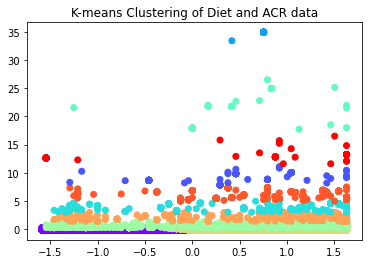
\includegraphics[scale=0.6]{images/kmeans/cluster-plot.png} \\
\end{tabular}
\caption{\textbf{10 Clusters created with KMeans Algorithm}}
\label{cluster-plot}
\vspace{0.25cm}
\end{figure}

\begin{figure}
\begin{tabular}{c}
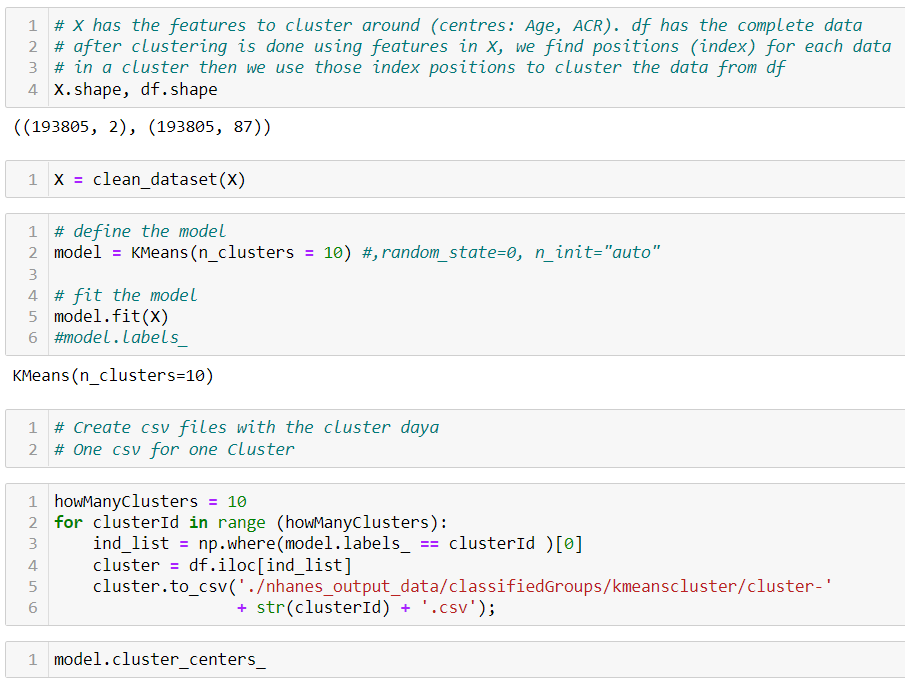
\includegraphics[scale=0.6]{images/kmeans/kmeans-clustering-implementations.png} \\
\end{tabular}
\caption{\textbf{KMeans Code for Clustering }}
\label{kmeans-python}
\vspace{0.25cm}
\end{figure}